% --- APA 7 para todas las figuras ---
% Figura 2
\begin{figure}[htbp]
    \begin{flushleft}
        \textbf{Figura 2}\\
        \textit{Distribución global de la producción científica en el área de estudio}
    \end{flushleft}
    \centering
    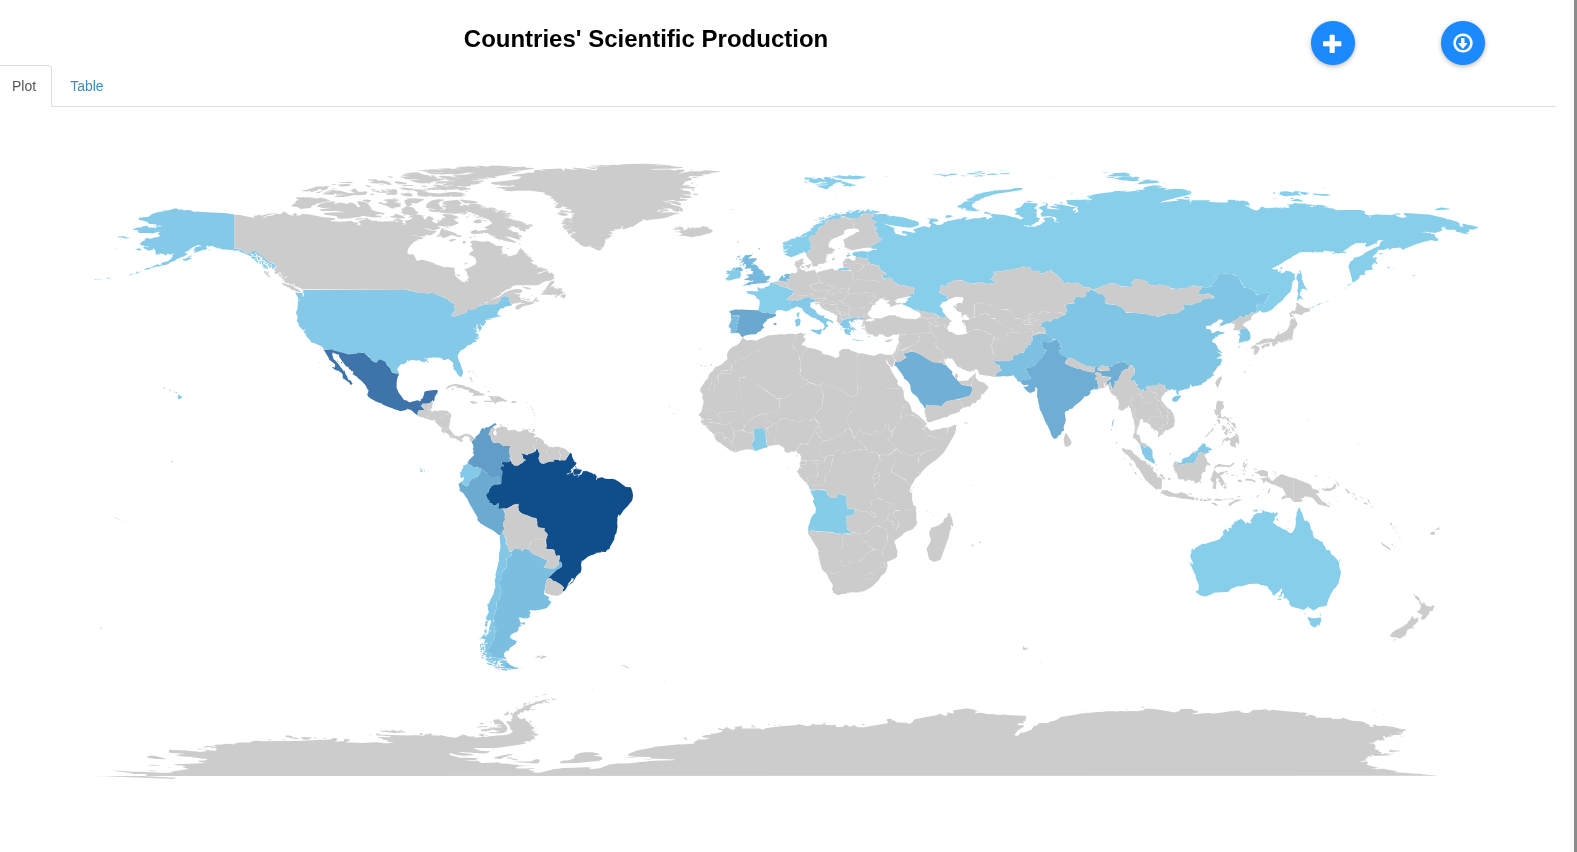
\includegraphics[width=0.8\textwidth]{Images/MapaBibliometrix.png}
    \vspace{0.5em}
    \begin{flushleft}
        \textit{Nota.} Tomado de Bibliometrix.
    \end{flushleft}
    \label{fig:mapa_bibliometrix}
\end{figure}

% Figura 3
\begin{figure}[htbp]
    \begin{flushleft}
        \textbf{Figura 3}\\
        \textit{Evolución de la producción científica a lo largo del tiempo por países}
    \end{flushleft}
    \centering
    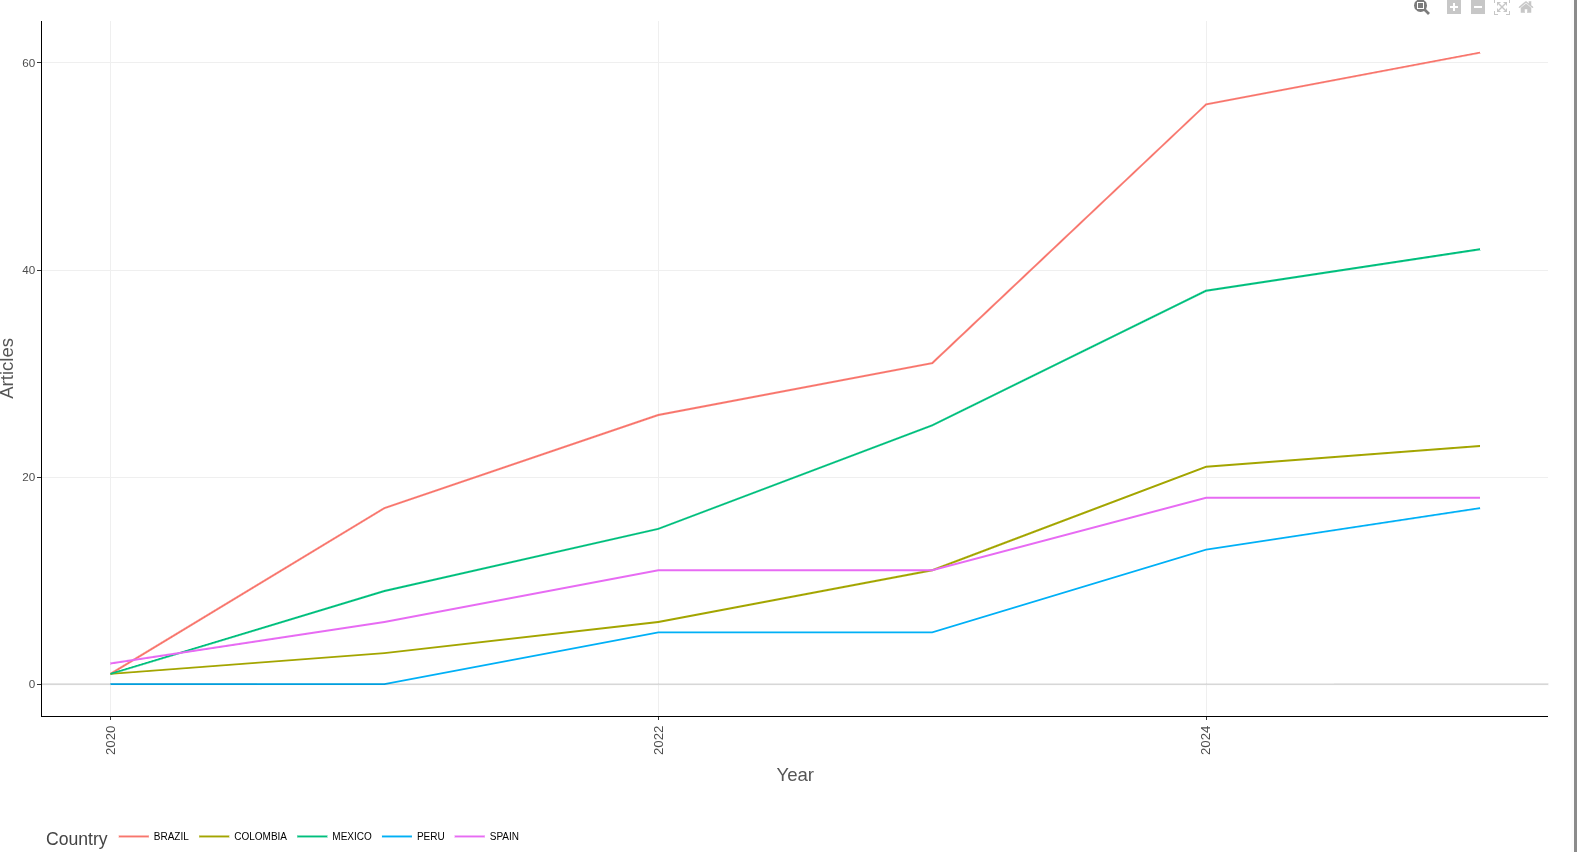
\includegraphics[width=0.8\textwidth]{Images/GraficoLineas.png}
    \vspace{0.5em}
    \begin{flushleft}
        \textit{Nota.} Tomado de Bibliometrix.
    \end{flushleft}
    \label{fig:grafico_lineas}
\end{figure}

% Figura 4
\begin{figure}[htbp]
    \begin{flushleft}
        \textbf{Figura 4}\\
        \textit{Nube de palabras que representa la frecuencia de términos en la literatura analizada}
    \end{flushleft}
    \centering
    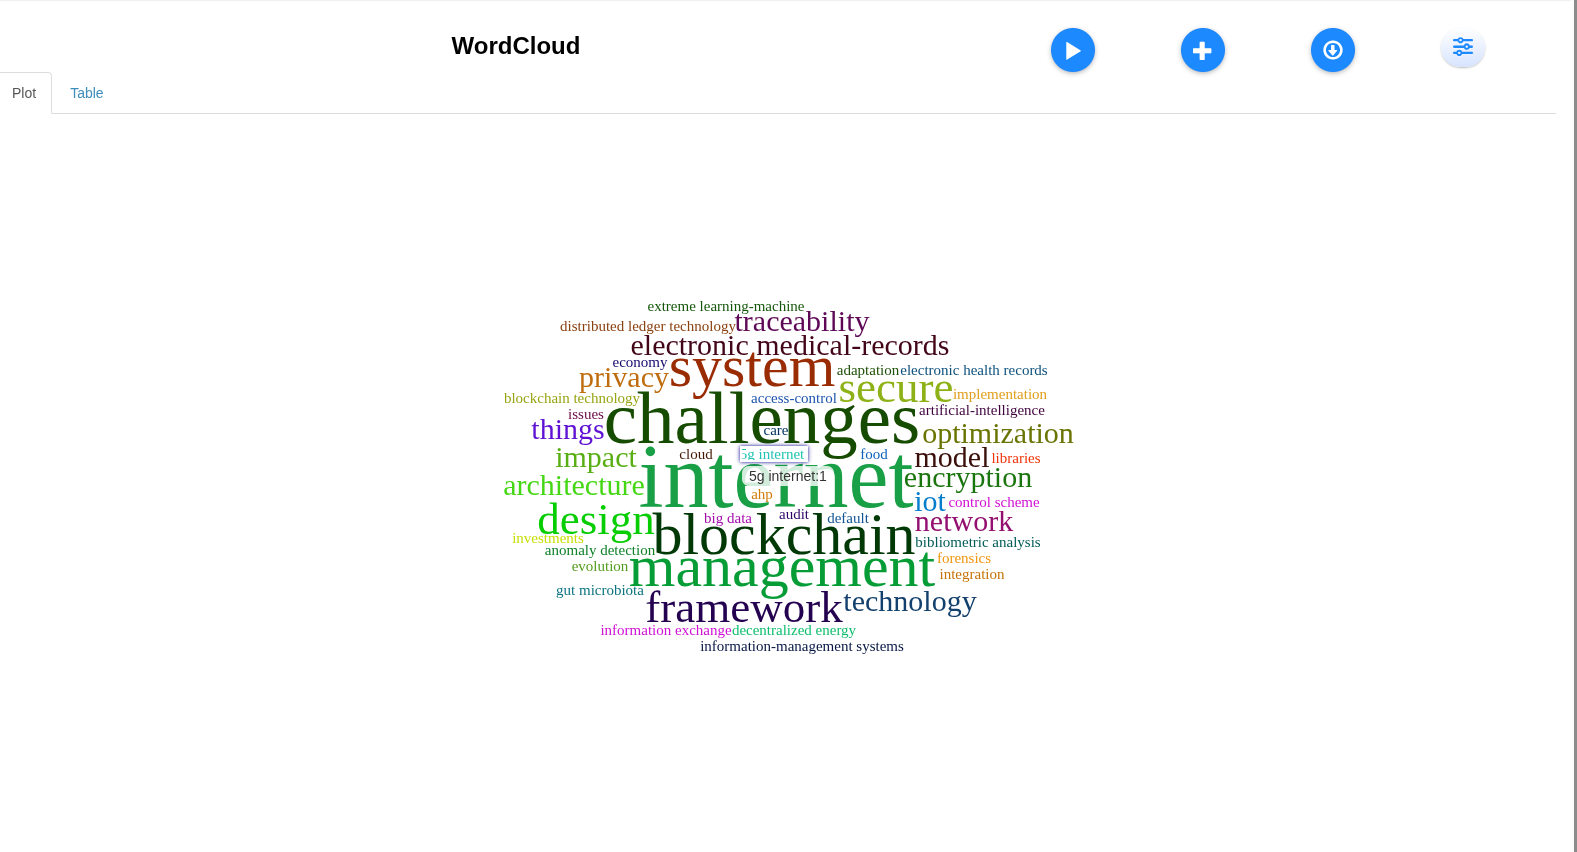
\includegraphics[width=0.8\textwidth]{Images/NubePalabras.png}
    \vspace{0.5em}
    \begin{flushleft}
        \textit{Nota.} Tomado de Bibliometrix.
    \end{flushleft}
    \label{fig:nube_palabras}
\end{figure}

% Figura 5
\begin{figure}[htbp]
    \begin{flushleft}
        \textbf{Figura 5}\\
        \textit{Mapa temático que clasifica los temas de investigación según centralidad y densidad}
    \end{flushleft}
    \centering
    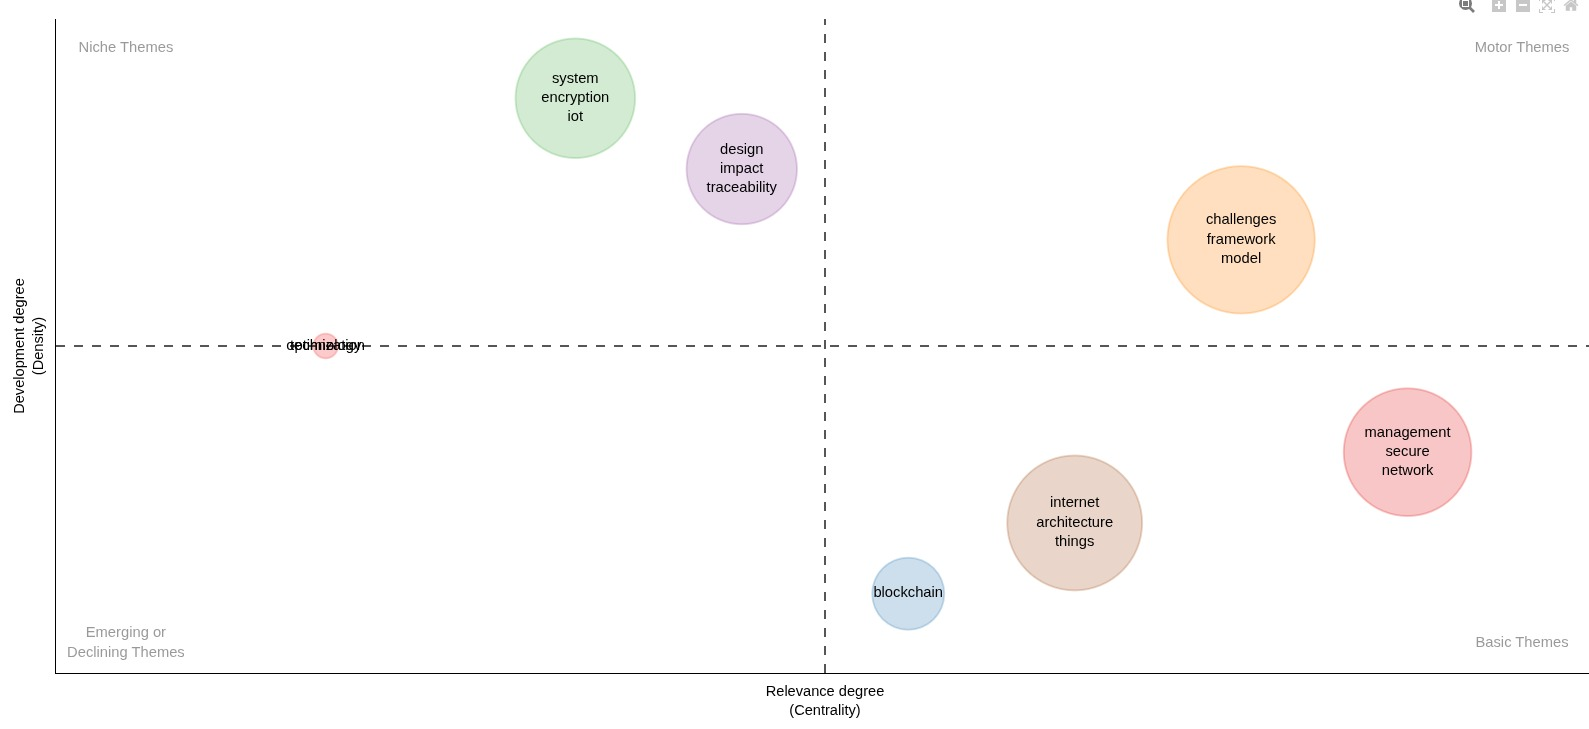
\includegraphics[width=0.8\textwidth]{Images/MapaTematico.jpeg}
    \vspace{0.5em}
    \begin{flushleft}
        \textit{Nota.} Tomado de Bibliometrix.
    \end{flushleft}
    \label{fig:mapa_tematico}
\end{figure}

% Figura 6
\begin{figure}[htbp]
    \begin{flushleft}
        \textbf{Figura 6}\\
        \textit{Diagrama de casos de uso del sistema de gestión de infracciones de tránsito}
    \end{flushleft}
    \centering
    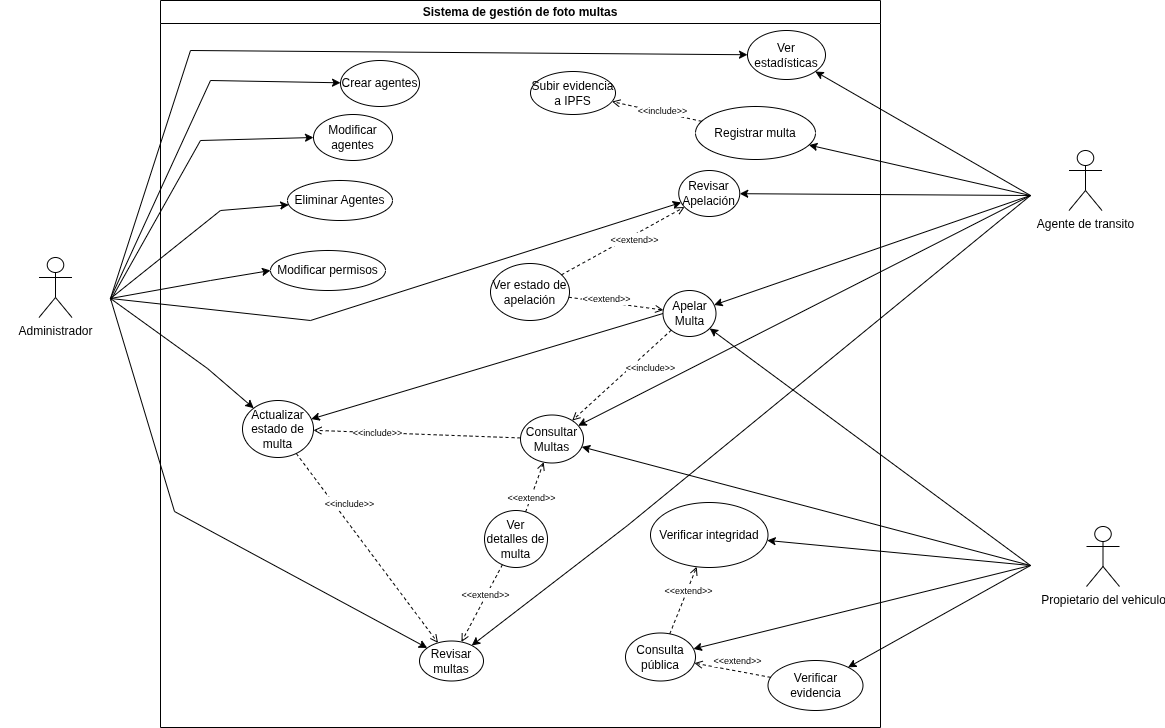
\includegraphics[width=0.8\textwidth]{Images/CasosUso.png}
    \vspace{0.5em}
    \begin{flushleft}
        \textit{Nota.} Elaboración propia.
    \end{flushleft}
    \label{fig:casos_uso}
\end{figure}

% Figura 7
\begin{figure}[htbp]
    \begin{flushleft}
        \textbf{Figura 7}\\
        \textit{Diagrama de despliegue de la arquitectura del sistema}
    \end{flushleft}
    \centering
    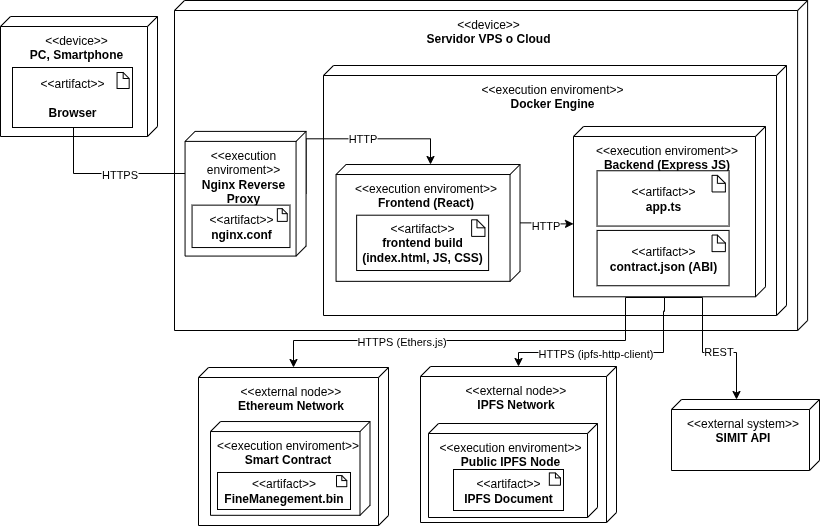
\includegraphics[width=0.8\textwidth]{Images/Despliegue.png}
    \vspace{0.5em}
    \begin{flushleft}
        \textit{Nota.} Elaboración propia.
    \end{flushleft}
    \label{fig:diagrama_despliegue}
\end{figure}

% Figura 8
\begin{figure}[htbp]
    \begin{flushleft}
        \textbf{Figura 8}\\
        \textit{Diagrama de clases del sistema de gestión de multas}
    \end{flushleft}
    \centering
    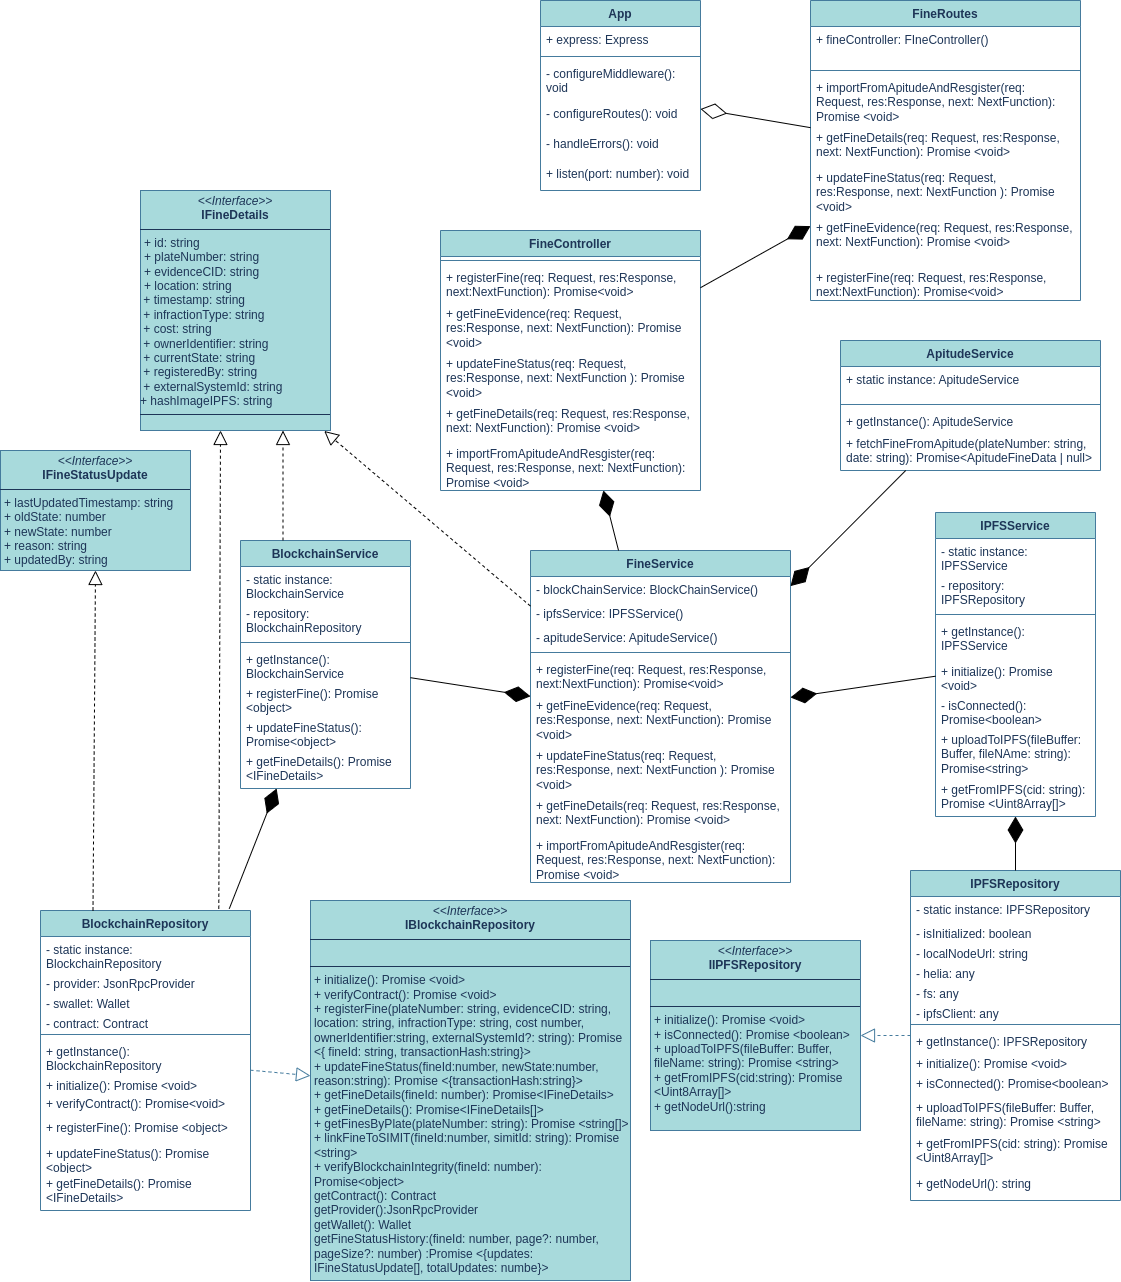
\includegraphics[width=0.8\textwidth]{Images/uml.png}
    \vspace{0.5em}
    \begin{flushleft}
        \textit{Nota.} Elaboración propia.
    \end{flushleft}
    \label{fig:diagrama_clases}
\end{figure}

% Figura 9
\begin{figure}[htbp]
    \begin{flushleft}
        \textbf{Figura 9}\\
        \textit{Diagrama de actividades para el proceso de apelación de multa}
    \end{flushleft}
    \centering
    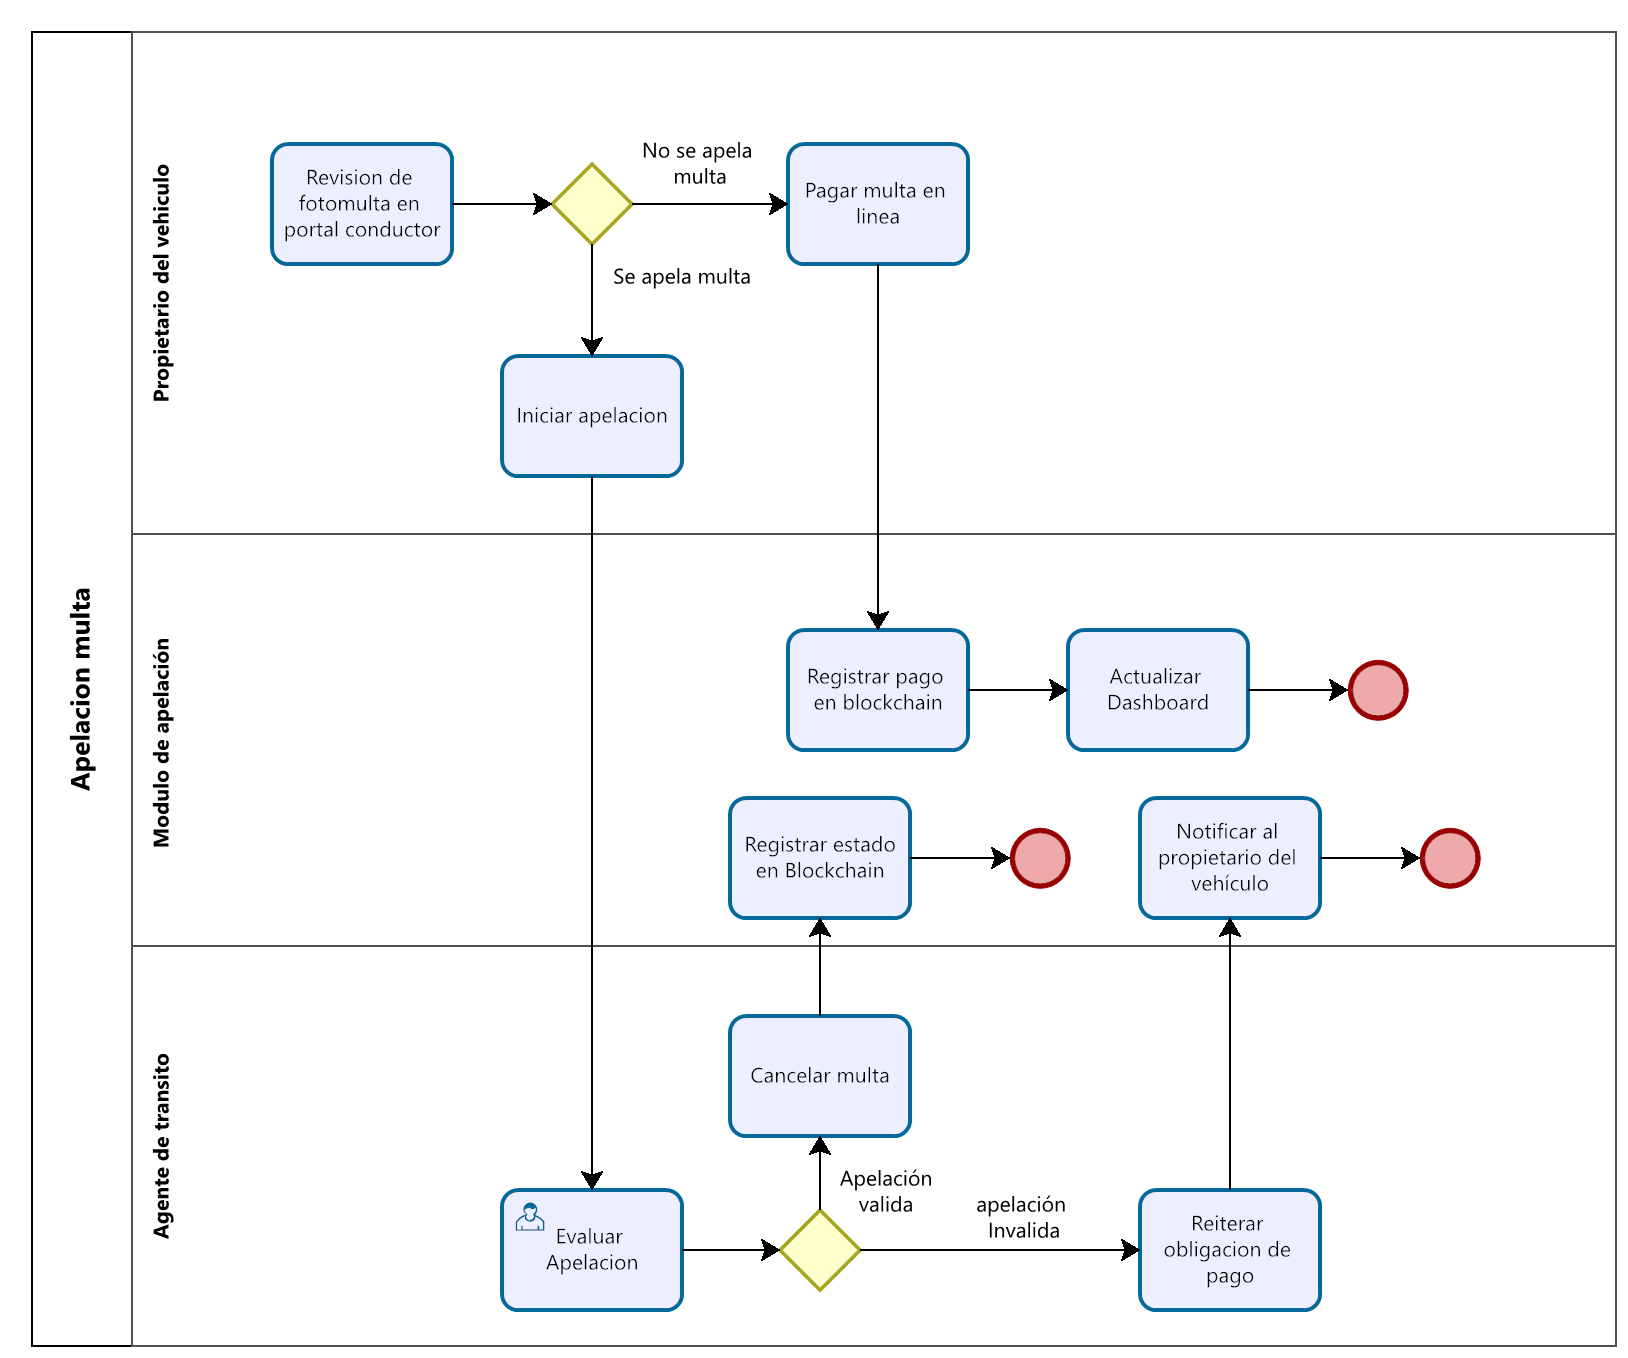
\includegraphics[width=0.8\textwidth]{Images/ActApelacion.png}
    \vspace{0.5em}
    \begin{flushleft}
        \textit{Nota.} Elaboración propia.
    \end{flushleft}
    \label{fig:diagrama_apelacion}
\end{figure}

% Figura 10
\begin{figure}[htbp]
    \begin{flushleft}
        \textbf{Figura 10}\\
        \textit{Diagrama de actividades para el proceso de creación de multa}
    \end{flushleft}
    \centering
    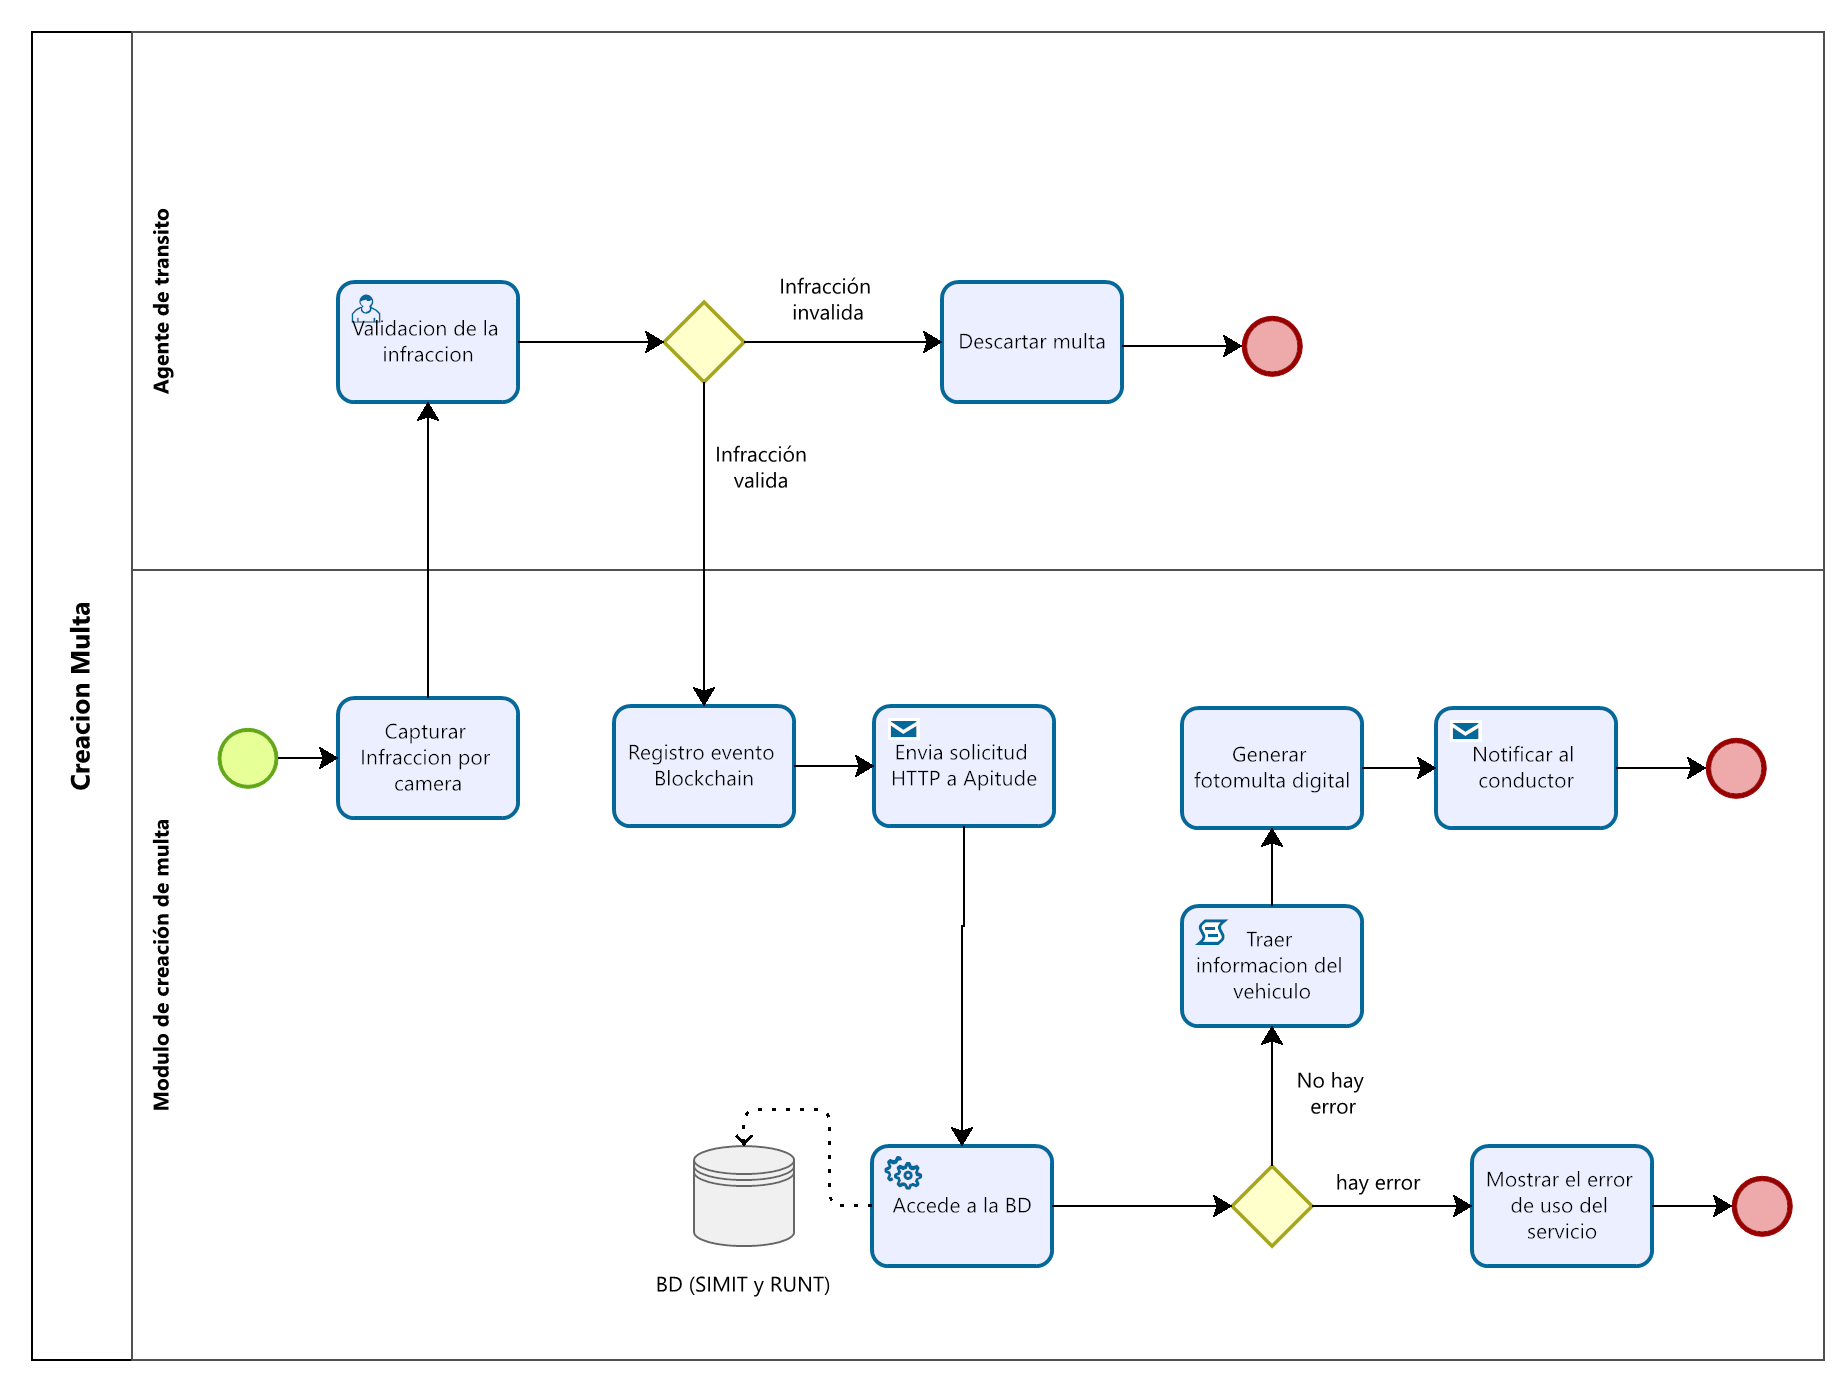
\includegraphics[width=0.8\textwidth]{Images/ActMulta.png}
    \vspace{0.5em}
    \begin{flushleft}
        \textit{Nota.} Elaboración propia.
    \end{flushleft}
    \label{fig:diagrama_creacion_multa}
\end{figure}

% Figura 11
\begin{figure}[htbp]
    \begin{flushleft}
        \textbf{Figura 11}\\
        \textit{Diagrama de actividades para el proceso de apelación de multa}
    \end{flushleft}
    \centering
    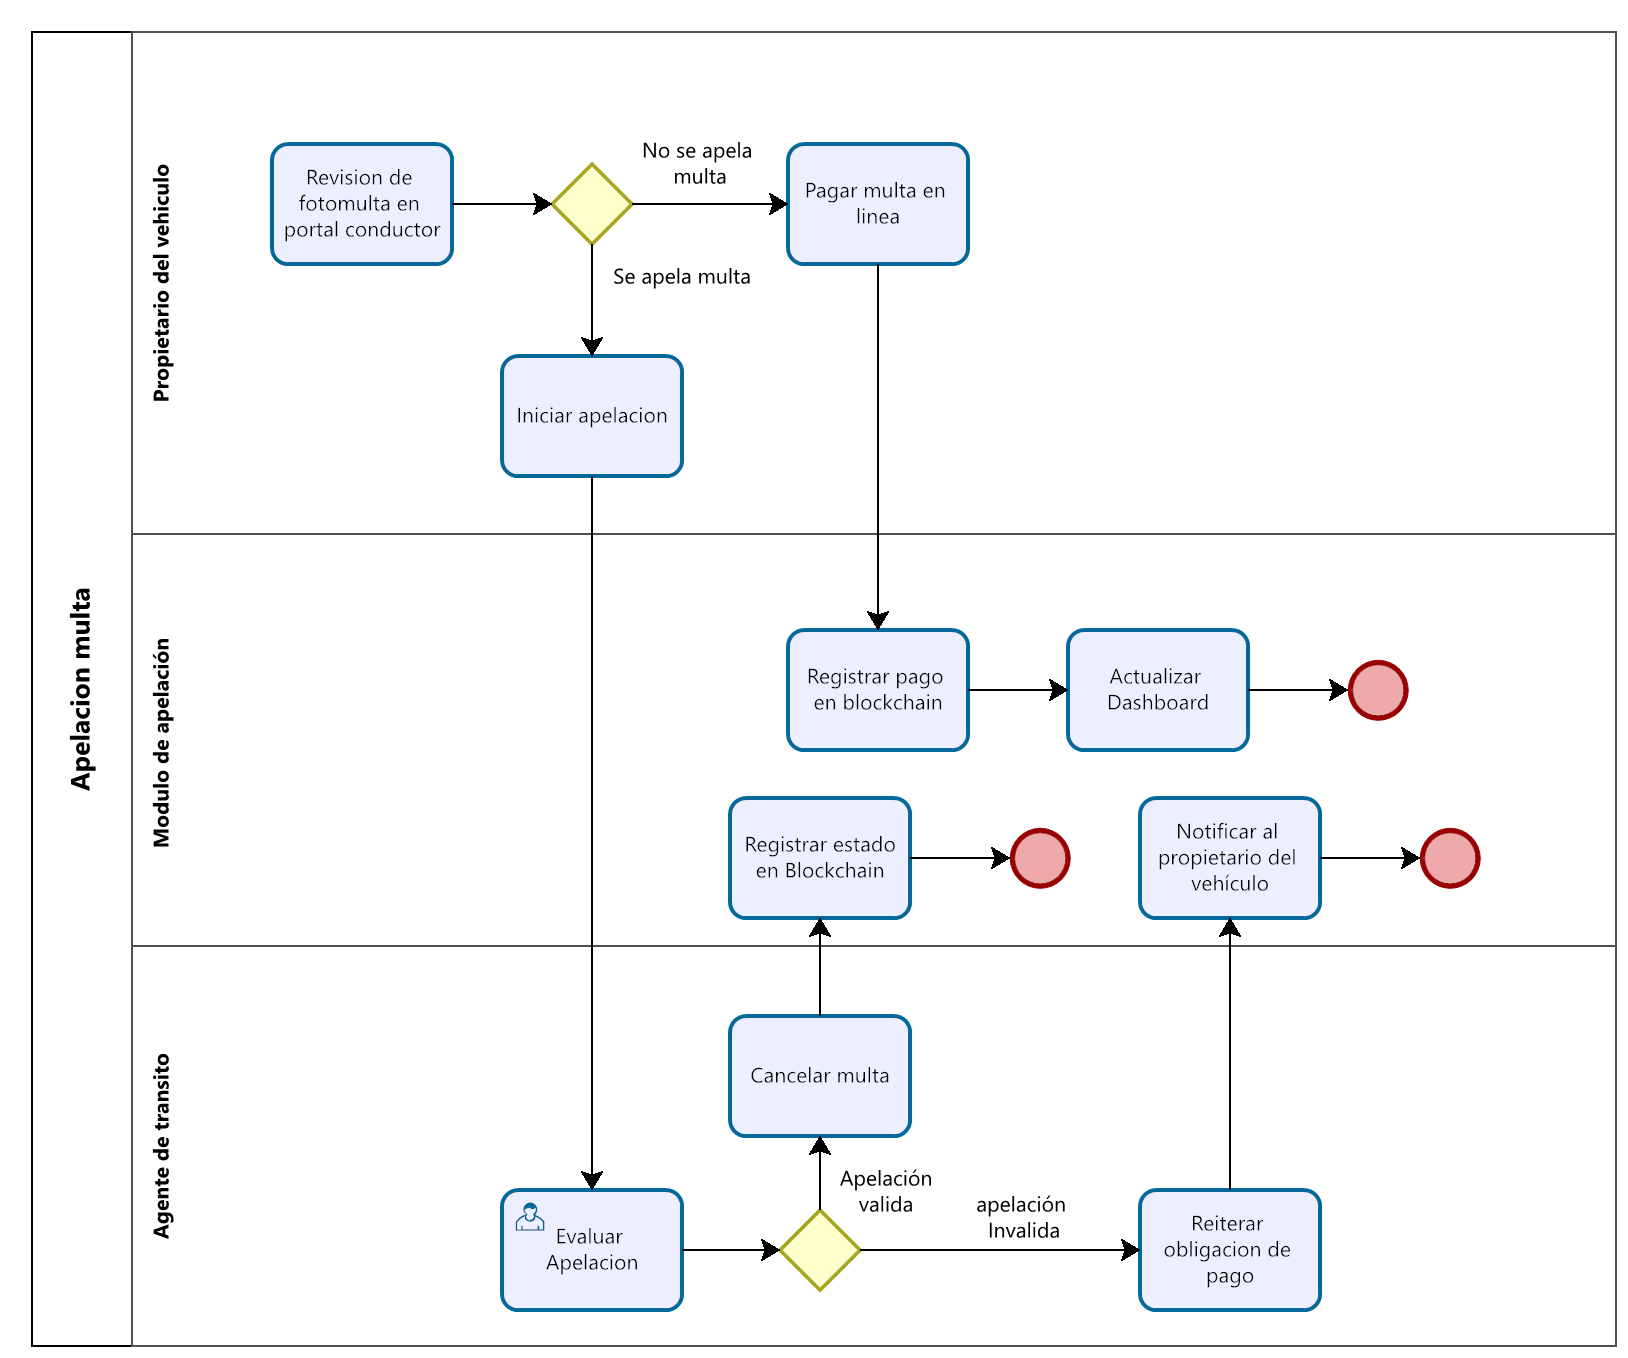
\includegraphics[width=0.8\textwidth]{Images/ActApelacion.png}
    \vspace{0.5em}
    \begin{flushleft}
        \textit{Nota.} Elaboración propia.
    \end{flushleft}
    \label{fig:diagrama_apelacion_2}
\end{figure}

% Figura 12
\begin{figure}[htbp]
    \begin{flushleft}
        \textbf{Figura 12}\\
        \textit{Pantalla de login del sistema}
    \end{flushleft}
    \centering
    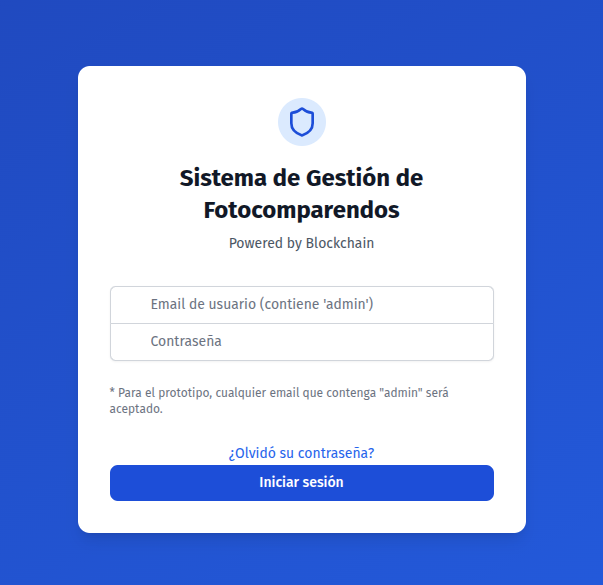
\includegraphics[width=0.8\textwidth]{Images/UI1.png}
    \vspace{0.5em}
    \begin{flushleft}
        \textit{Nota.} Elaboración propia.
    \end{flushleft}
    \label{fig:login}
\end{figure}

% Figura 13
\begin{figure}[htbp]
    \begin{flushleft}
        \textbf{Figura 13}\\
        \textit{Pantalla de recuperación de contraseña}
    \end{flushleft}
    \centering
    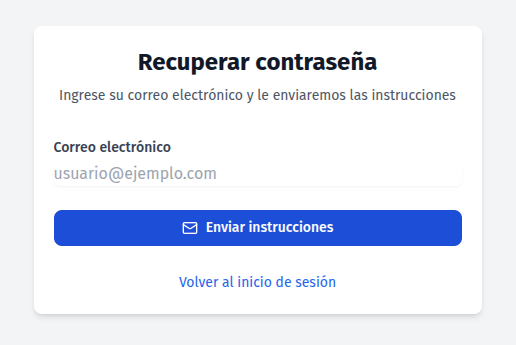
\includegraphics[width=0.8\textwidth]{Images/UI2.png}
    \vspace{0.5em}
    \begin{flushleft}
        \textit{Nota.} Elaboración propia.
    \end{flushleft}
    \label{fig:recuperar_password}
\end{figure}

% Figura 14
\begin{figure}[htbp]
    \begin{flushleft}
        \textbf{Figura 14}\\
        \textit{Dashboard del agente de tránsito}
    \end{flushleft}
    \centering
    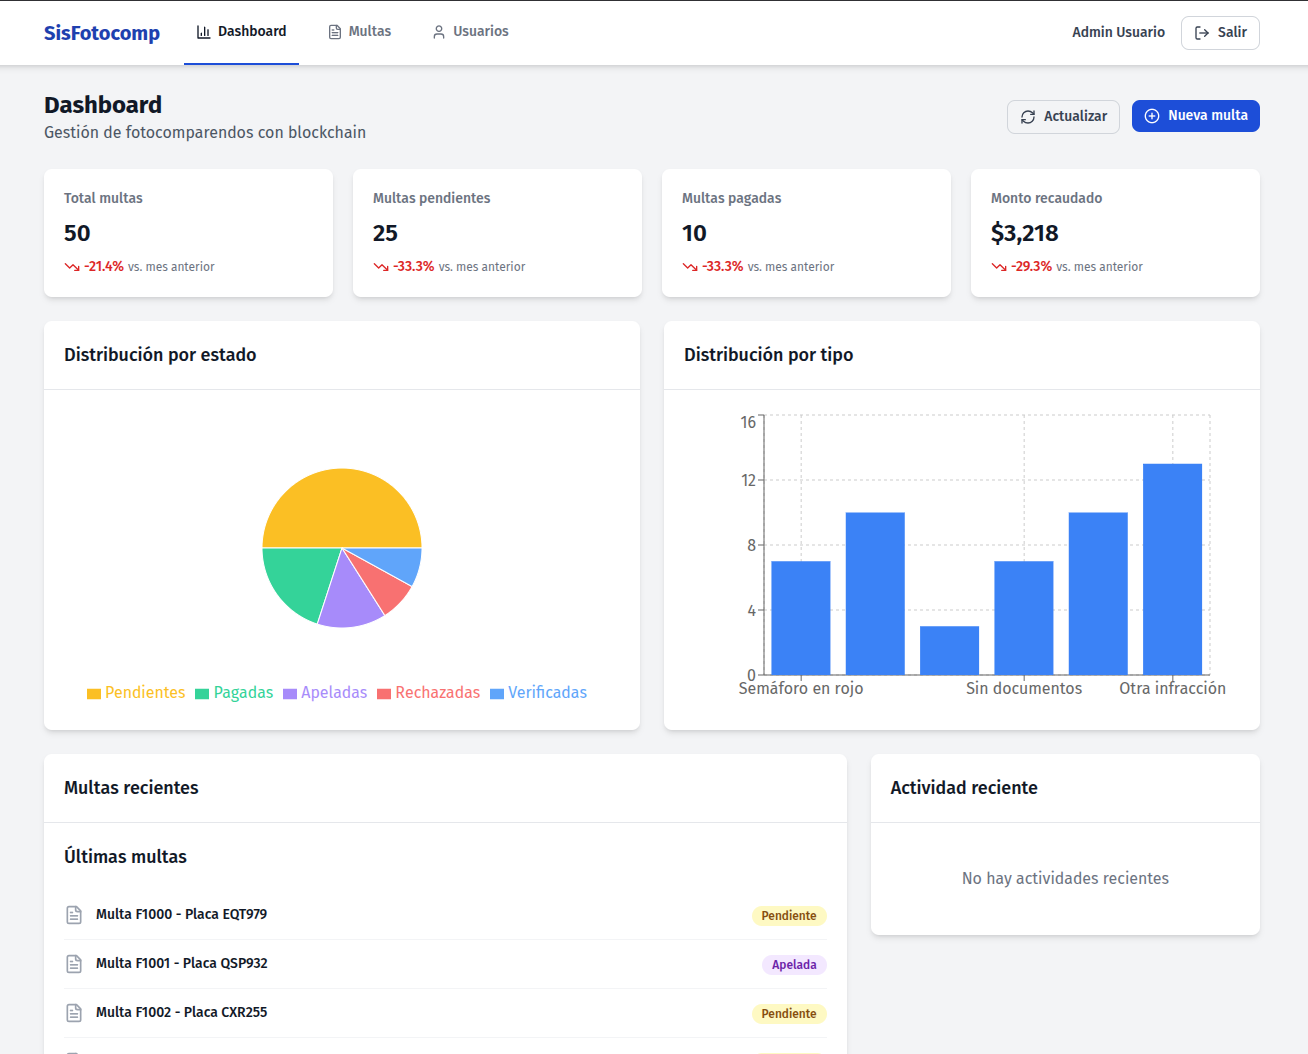
\includegraphics[width=0.8\textwidth]{Images/UI3.png}
    \vspace{0.5em}
    \begin{flushleft}
        \textit{Nota.} Elaboración propia.
    \end{flushleft}
    \label{fig:dashboard_agente}
\end{figure}

% Figura 15
\begin{figure}[htbp]
    \begin{flushleft}
        \textbf{Figura 15}\\
        \textit{Pantalla de consulta del estado de multa}
    \end{flushleft}
    \centering
    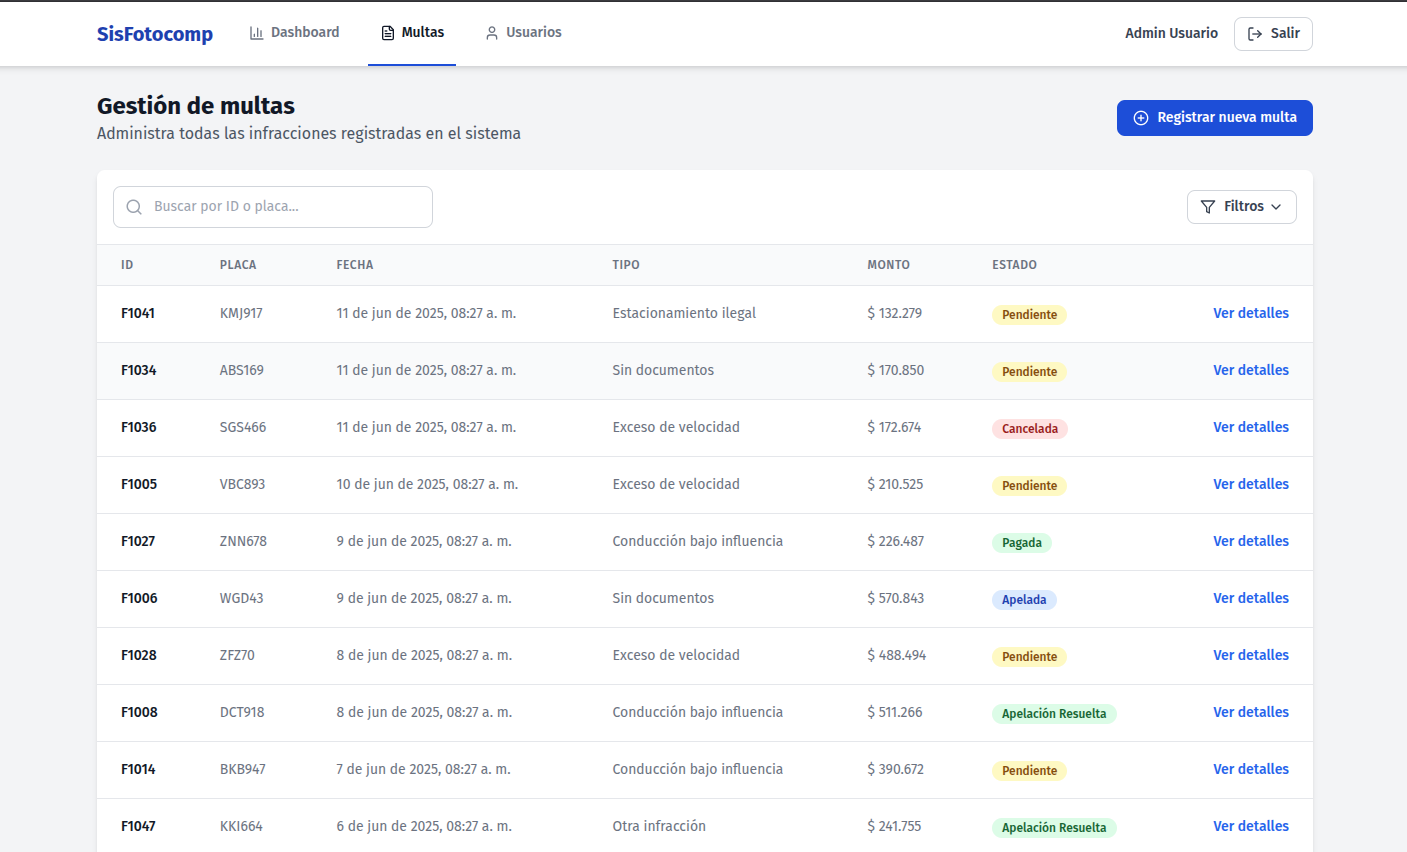
\includegraphics[width=0.8\textwidth]{Images/UI4.png}
    \vspace{0.5em}
    \begin{flushleft}
        \textit{Nota.} Elaboración propia.
    \end{flushleft}
    \label{fig:consulta_estado_multa}
\end{figure}

% Figura 16
\begin{figure}[htbp]
    \begin{flushleft}
        \textbf{Figura 16}\\
        \textit{Pantalla de consulta de detalle de multa}
    \end{flushleft}
    \centering
    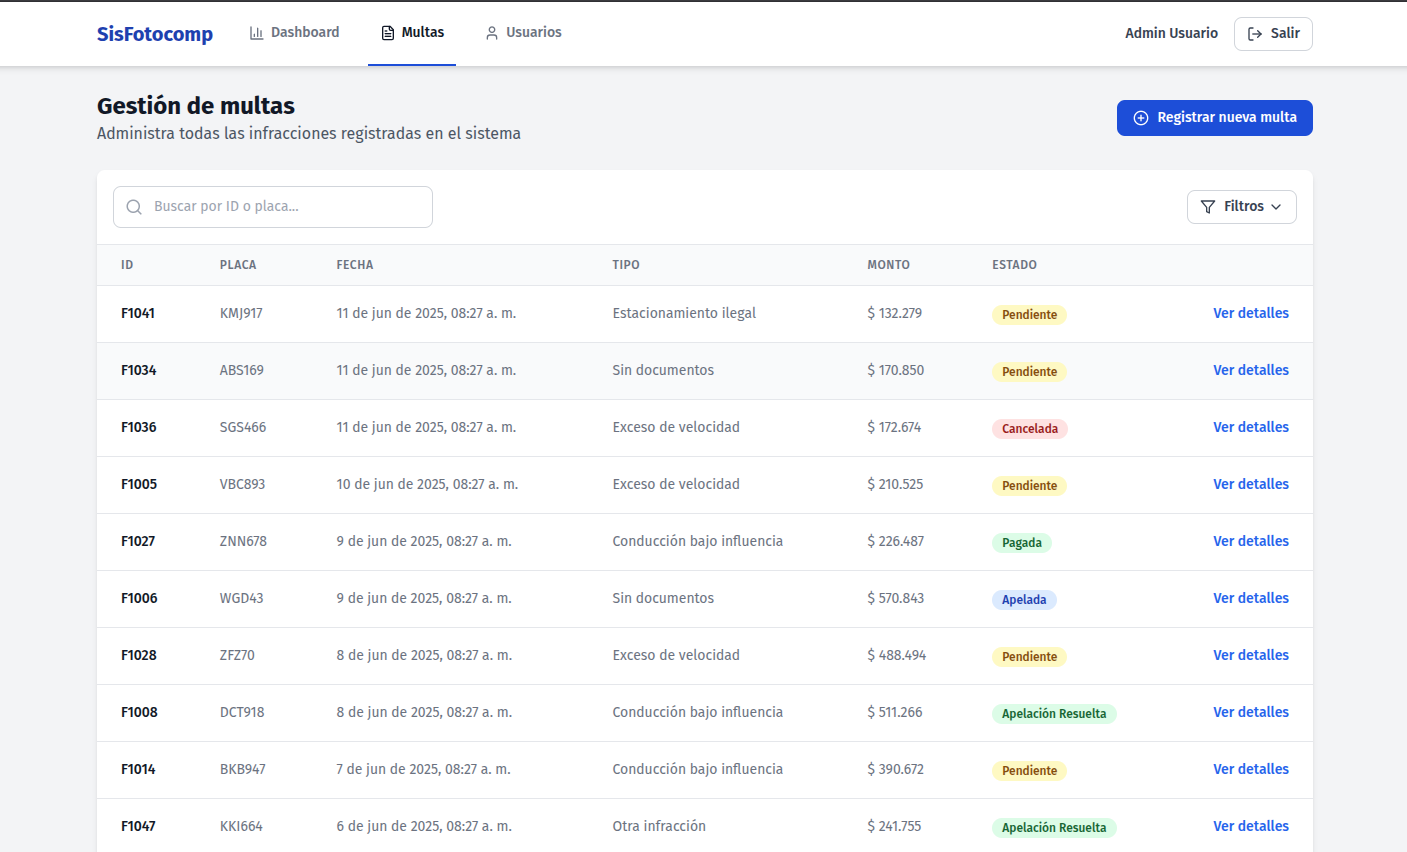
\includegraphics[width=0.8\textwidth]{Images/UI4.png}
    \vspace{0.5em}
    \begin{flushleft}
        \textit{Nota.} Elaboración propia.
    \end{flushleft}
    \label{fig:consulta_detalle_multa}
\end{figure}

% Figura 17
\begin{figure}[htbp]
    \begin{flushleft}
        \textbf{Figura 17}\\
        \textit{Pantalla de consulta de multas para propietarios de vehículos}
    \end{flushleft}
    \centering
    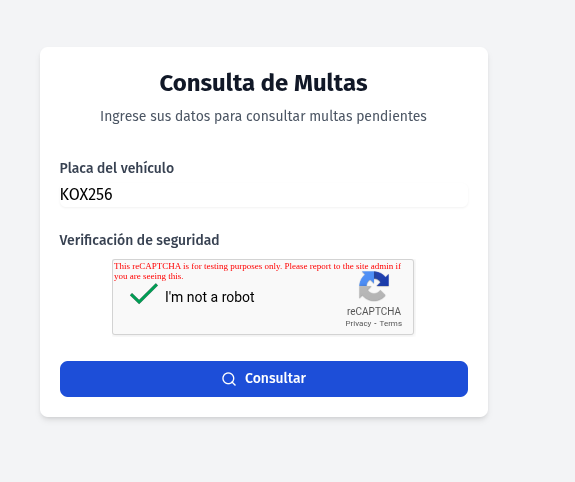
\includegraphics[width=0.8\textwidth]{Images/UI5.png}
    \vspace{0.5em}
    \begin{flushleft}
        \textit{Nota.} Elaboración propia.
    \end{flushleft}
    \label{fig:consulta_multas_propietario}
\end{figure}

% Figura 18
\begin{figure}[htbp]
    \begin{flushleft}
        \textbf{Figura 18}\\
        \textit{Resumen de costos del proyecto}
    \end{flushleft}
    \centering
    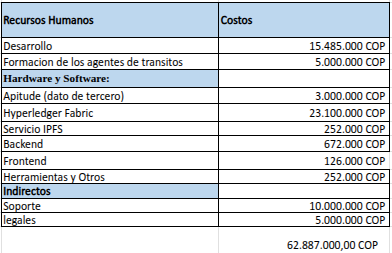
\includegraphics[width=\textwidth]{Images/costos1.png}
    \vspace{0.5em}
    \begin{flushleft}
        \textit{Nota.} Elaboración propia.
    \end{flushleft}
    \label{fig:costos1}
\end{figure}

% Figura 19
\begin{figure}[htbp]
    \begin{flushleft}
        \textbf{Figura 19}\\
        \textit{Estimación de costos mensuales de infraestructura}
    \end{flushleft}
    \centering
    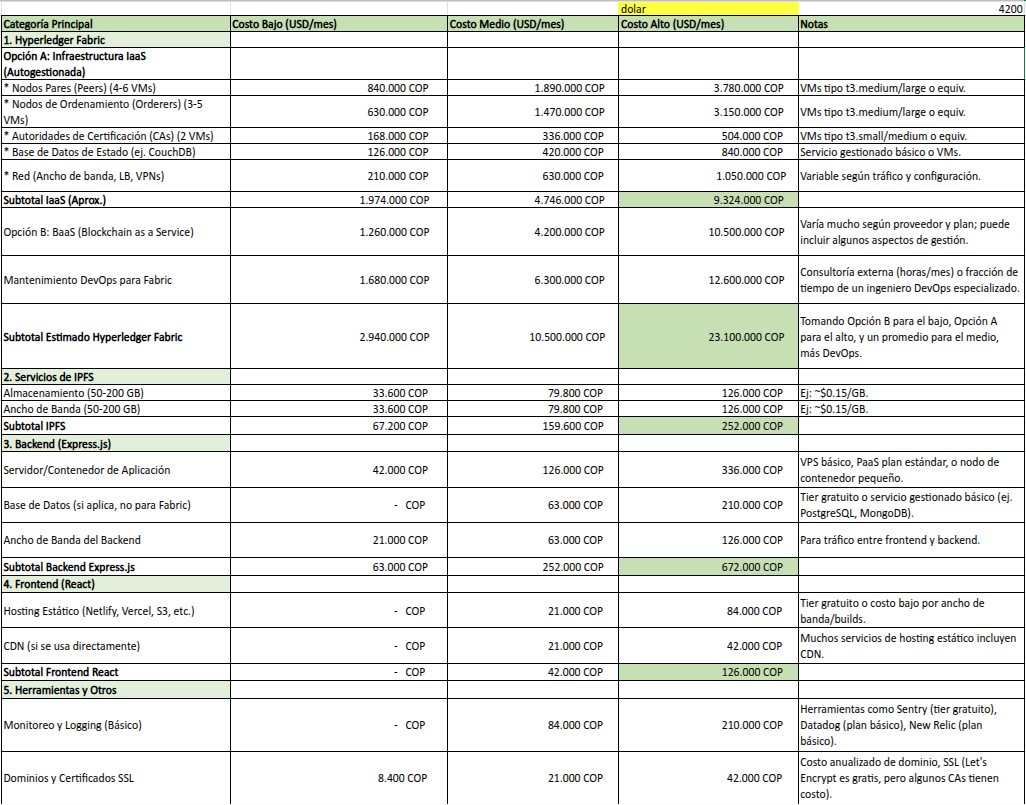
\includegraphics[width=\textwidth]{Images/costos2.png}
    \vspace{0.5em}
    \begin{flushleft}
        \textit{Nota.} Elaboración propia.
    \end{flushleft}
    \label{fig:costos2}
\end{figure}

% Figura 20
\begin{figure}[htbp]
    \begin{flushleft}
        \textbf{Figura 20}\\
        \textit{Estimación de costos de desarrollo del proyecto}
    \end{flushleft}
    \centering
    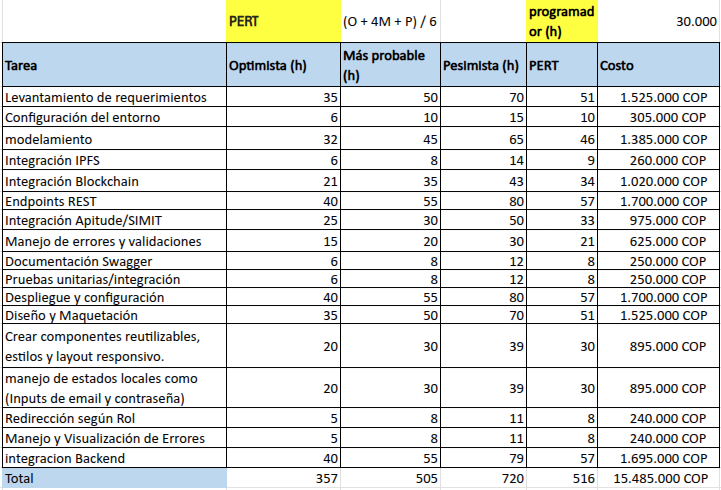
\includegraphics[width=\textwidth]{Images/costos3.png}
    \vspace{0.5em}
    \begin{flushleft}
        \textit{Nota.} Elaboración propia.
    \end{flushleft}
    \label{fig:costos3}
\end{figure} 